O sol sobe mais um palmo no céu e as flores mais dorminhocas só agora começam a abrir as pétalas na sua direção.

As gotículas de água dentro delas, escorrem e pingam na terra junto ao seu caule. É assim que as flores lavam a cara logo pela manhã.

É neste momento que a bola dançarina e flutuante pousa em frente do plenário dos insetos. E não faz Ploc.

Fica durante uns segundos a mudar de cor, a mesclar as cores, a avivá-las até que se torna azul, estática e silenciosa.

Os insetos silenciosos ficaram. Ninguém se mexe, nem pestaneja.

Um canteiro de girassóis, que são aquelas flores que sorriem o dia inteiro na direção do sol, retorcem as suas hastes para também poderem ver o que está a acontecer.

E a passarada, deixando de gorjear, recolhe-se nos ramos da árvore vigilante, mesmo em frente da misteriosa bola azul.
\bigbreak
— Ssssssssssssssssss...
\bigbreak
Ouve-se um sibilo parecido com o zunir dos insetos, mas mais melodioso.

Uma abertura começa a surgir na parte da bola virada para os observadores de olhos arregalados.

E o mais engraçado é que essa abertura dá a volta a toda a superfície da esfera e desaparece no lado oposto. A bola simplesmente some.

No seu lugar fica um pequeno ser, cuja estatura cabe na palma da mão de uma criança.

Não! Não pode ser deste mundo o que está a acontecer. Mas ao mesmo tempo não é nada assustador.
\bigbreak
O pequeno recém-chegado tem um corpo com características humanas - cabeça, tronco e membros. Tem um rosto amendoado e olhos bem grandes e escuros. As orelhas são pontiagudas e pequeninas. O nariz é arrebitado e as bochechas dão um ar engraçado à expressão facial do visitante, sempre sorridente. Está vestido com um traje inteiro e prateado, luvas e botas da mesma cor. E agora, o mais interessante. A cor da pele deste pequeno ser é azul, da cor do céu ou do mar, tanto faz, porque é sempre maravilhosa. Mais um pormenor. Na sua cabeça tem um pequeno chapéu-capacete, com uma única antena, deixando visíveis as orelhas. A antena não está quieta, sempre a tremelicar com os movimentos.
\bigbreak
— Quem és tu? – pergunta um dos insetos mais despachado.
\bigbreak
No jardim banhado pelo sol todos aguardam a resposta.
\bigbreak
— Eu... sou Eu! – responde o pequeno ser, rasgando um sorriso de orelha a orelha.
\bigbreak
O mar dos bicharocos avança um passo em frente, atraído pela curiosidade.

\begin{figure}[h]
    \centering
    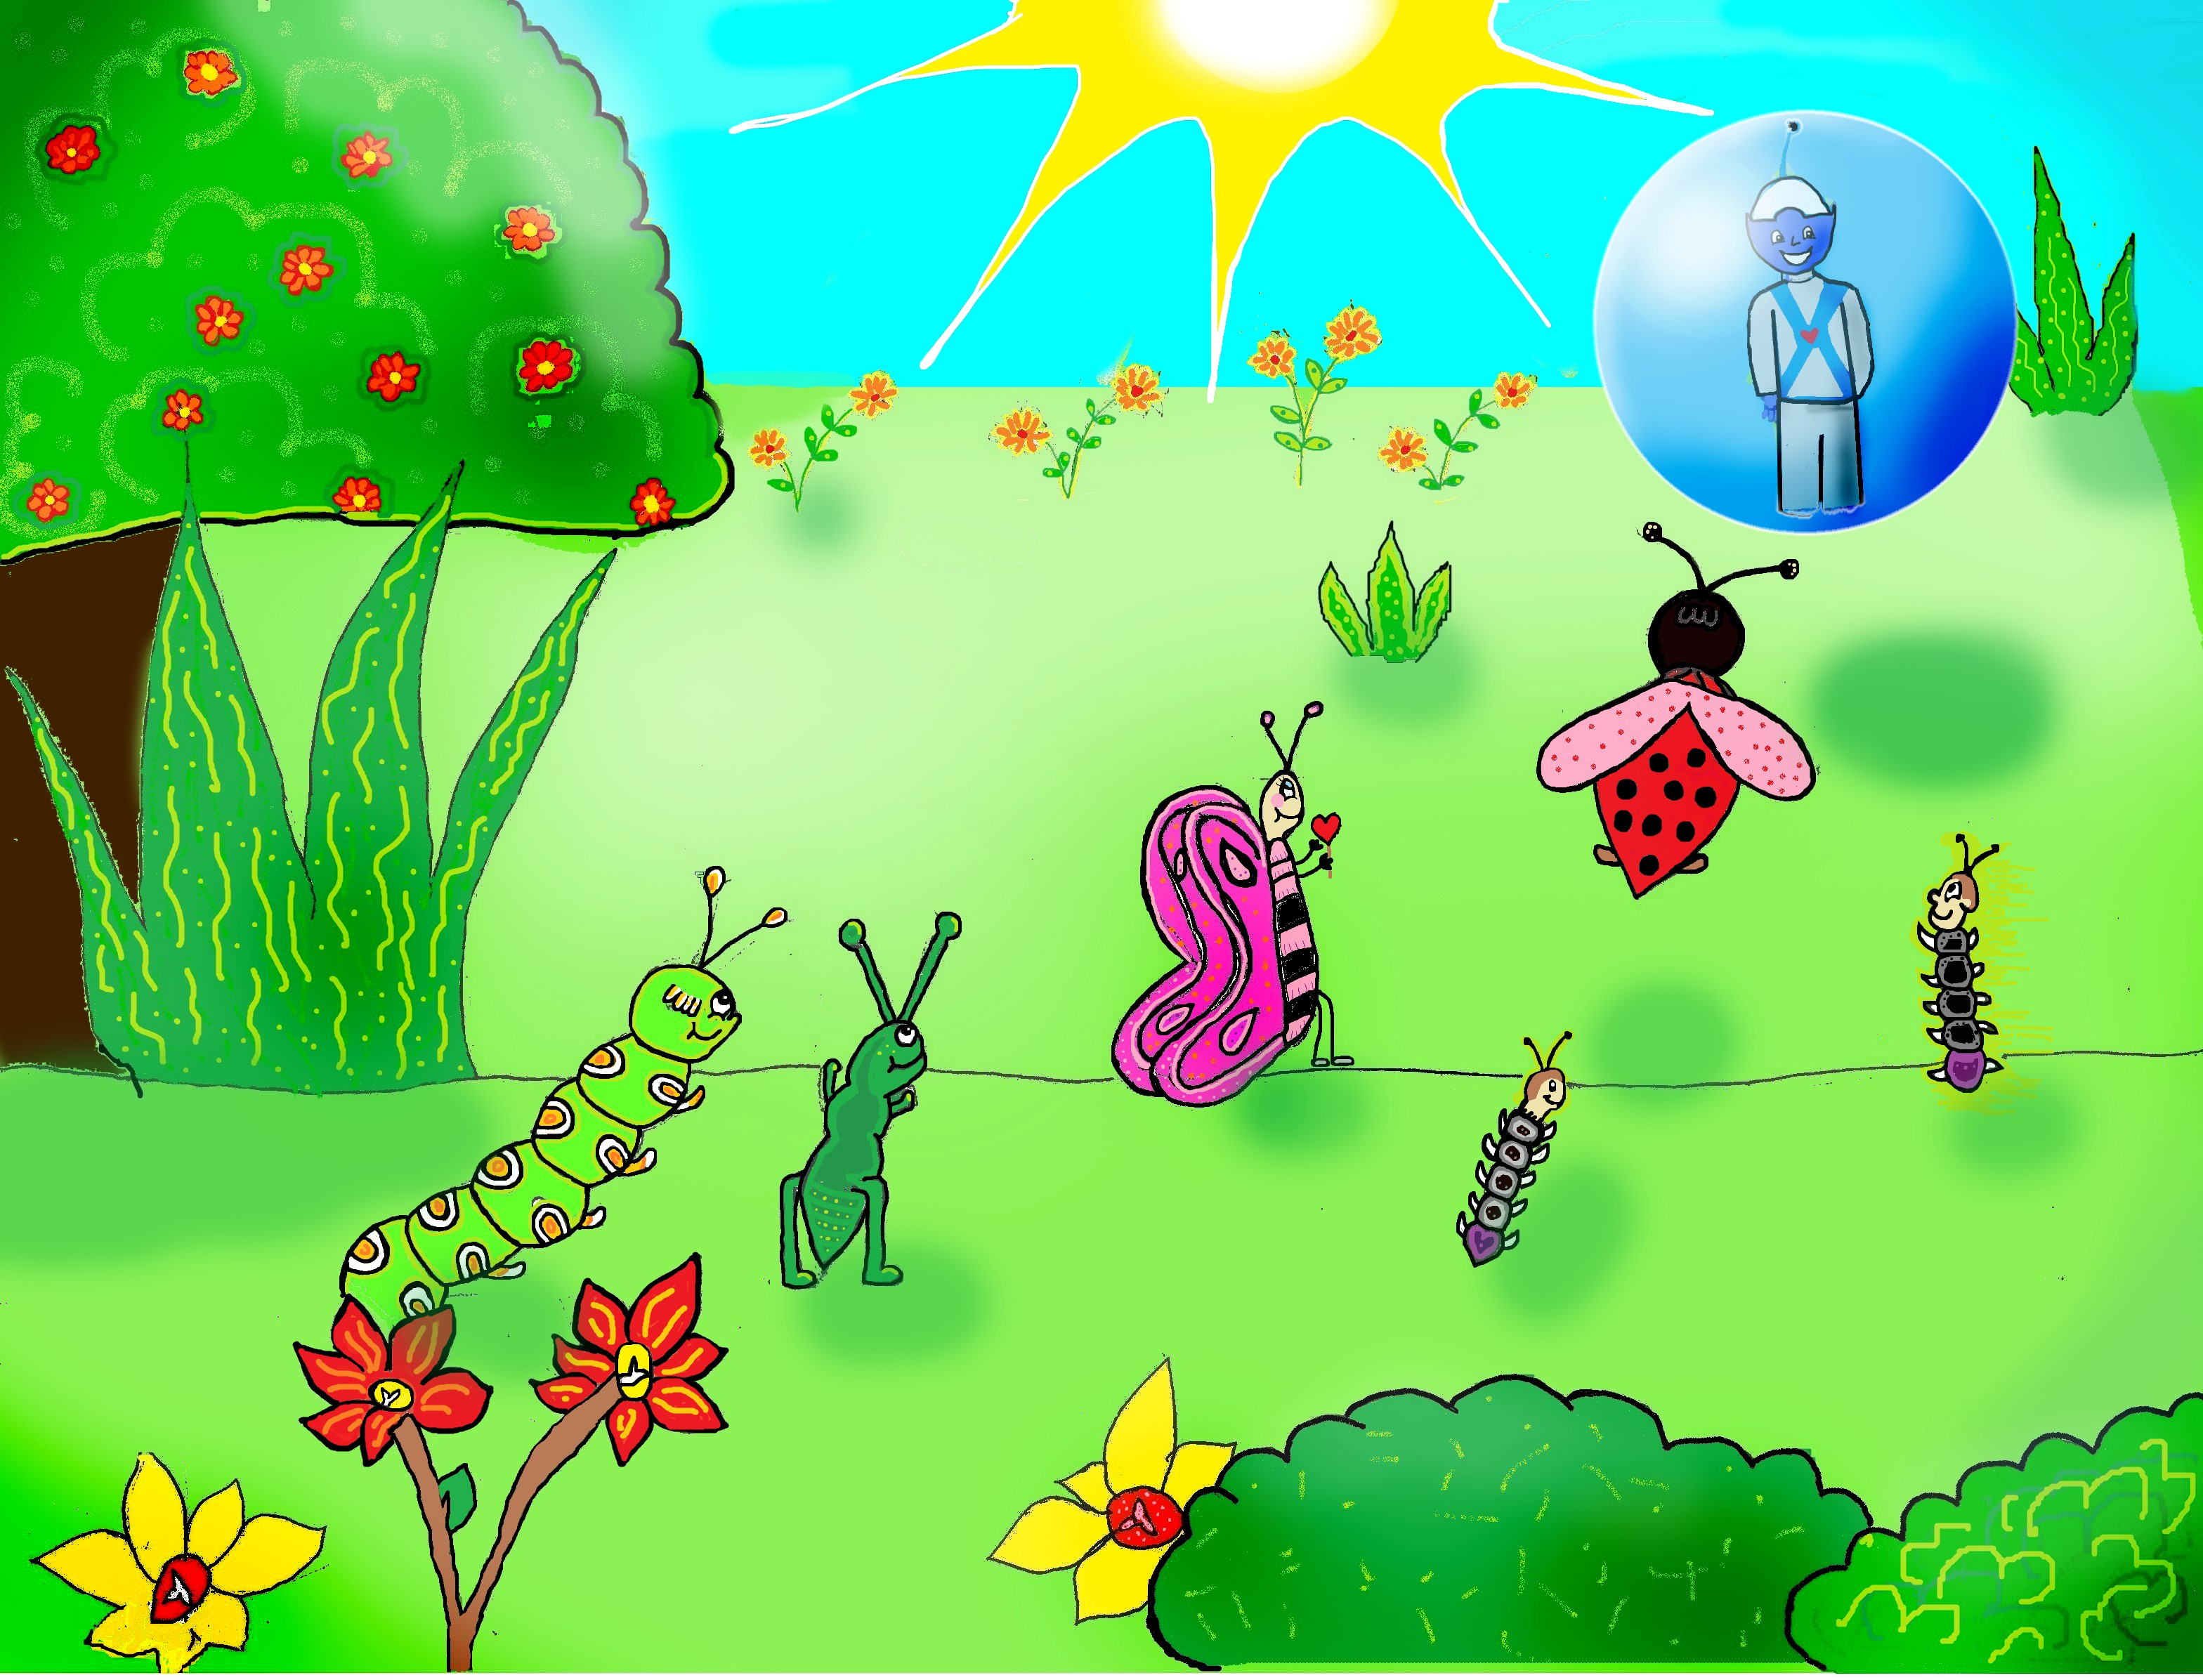
\includegraphics[width=0.75\textwidth]{bolha}
\end{figure}

— Qual é o teu nome? De onde vens? O que vieste fazer aqui? – pergunta uma lagarta trapalhona, verde e rechonchuda.
\bigbreak
Um burburinho tem início e o entusiasmo começa a aumentar. Querem todos fazer perguntas sem fim e ao mesmo tempo.

O jardim está mais vivo do que nunca, porque não há ninguém que não queira perceber quem é o \textbf{Eu sou Eu}, recém aterrissado numa bola de sabão.

De modo a não se atrapalharem uns aos outros, rapidamente fica determinado que para perguntar basta levantar a pata no ar e o \textbf{Eu sou Eu} aponta o inseto questionador.

Mas antes de iniciar as respostas às “milhentas” questões que já borbulham, \textbf{Eu sou Eu} pede-lhes para fazer uma só pergunta:

— E vocês, como é que se chamam?

— Somos as lagartas!

— Somos as formigas!

— Somos as borboletas!

E assim, as pequenas criaturas vão levantando as patitas no ar e dando os seus nomes de conjunto.
\bigbreak
O \textbf{Eu sou Eu} dá uma gargalhada, faz uma pirueta e diz:
\bigbreak
— Veem?! Sintam! Vocês são Unidade porque quando se pergunta o nome respondem em União. É exatamente o que acontece no meu planeta. Todos somos chamados, mas sabemos quem é que precisa avançar aquando do chamamento. Assim estamos sempre em sintonia e em prontidão. No meu mundo todos sabemos tudo ao mesmo tempo.
\bigbreak
\textbf{Eu sou Eu} continua com o esclarecimento:
\bigbreak
— Venho de AnThais, um planeta encantador que orbita Sírius, que é o nosso sol. Distancia-se daqui apenas 8,5 anos-luz, o que é bem perto.
\bigbreak
Bem perto, ora muito bem... vamos lá fazer as contas.
Se a velocidade da luz é 300.000 quilômetros por segundo, se 1 minuto tem 60 segundos, se 1 hora tem 60 minutos, se 1 dia tem 24 horas, se 1 mês tem 30 dias, se 1 ano tem 12 meses, andando de trás para frente e multiplicando tudo por oito e meio, isto dá qualquer coisa como 81 trilhões de quilômetros.

Humm!... 81 trilhões de quilômetros percorrem-se com um olhar no céu quando se observa uma estrela!

No final das contas não é longe.
\bigbreak
— Que fixe! É bem pertinho!

— Podemos ir lá?

— Sim! Vamos nas bolas de sabão.

— E se elas explodem na viagem?

— Não sejas pateta, são bolas especiais.

— Especiais e espaciais!

— Eu ando um metro e já fico cansada!

— Ficas cansada porque és uma lesma barriguda.

— Eu sou grande demais para entrar na bola de sabão!

O \textbf{Eu sou Eu} está divertidíssimo com tudo o que ouve. O entusiasmo é tal, que os insetos bisbilhotam uns com os outros e as conversas misturam-se.

Por um bom bocado de tempo esquecem-se do \textbf{Eu sou Eu} que se senta numa pedra, cruza as pernas e fica a observar o jardim.

O sol avança devagarinho no céu com os seus raios de luz a acariciar cada flor deste lugar.

De repente alguém pergunta:
\bigbreak
— Os habitantes de AnThais são todos como tu?
\bigbreak
Ora bem, aí está uma pergunta importante cuja resposta vai transportá-los a um mundo totalmente desconhecido.
\bigbreak
— Sim! – diz o \textbf{Eu sou Eu} – são todos como eu e todos diferentes de mim. Eu vou explicar. No meu planeta não há forma fixa. Temos Liberdade e Autonomia para sermos o que quisermos. Mas sempre em Unidade. Por exemplo, eu escolhi visitar o planeta Terra porque o achei engraçado e pequenino. Então, decidi a aparência que queria ter, as roupas que usaria, o local de pouso, os contatos imediatos e o veículo que me transportaria. Igualmente engraçado e agradável foi viajar numa Esfera Transdimensional. E assim aqui estou eu.
\bigbreak
Num clique faz-se luz na cabeça da multidão dos insetos.

Afinal não são bolinhas de sabão e nem tinham estado a lavar roupa no céu, mas são sim Esferas Transdimensionais.

O \textbf{Eu sou Eu} pode sentir o espanto dos insetos com a revelação. O panorama geral é de bocas abertas de admiração.

E as explicações continuam.
\bigbreak
— Uma Esfera Transdimensional é formada por um foco de energia que permite a fusão com quem se quer transportar. Este feixe energético é gerado por uma máquina muito simples que está ligada ao nosso sol – Sírius - e é acionada pelo pensamento. Quando decidimos viajar, basta informarmos os controladores espaciais do nosso desejo. Isto, porque todos os AnThaisianos são viajantes cósmicos e as plataformas de embarque são muito concorridas. Somos chamados na nossa vez. A Ordem e o Respeito fazem parte da nossa Essência. No dia do embarque podemos optar pela forma da nave, qualquer uma. Eu escolhi uma ET.
\bigbreak
— ET? – dizem os insetos em coro.

— ET - Esfera Transdimensional! – o \textbf{Eu sou Eu} sorri emanando carinho.
\bigbreak
Outra pergunta surge de imediato, feita por um dos insetos, mas que todos queriam fazê-la.
\bigbreak
— Mas como conseguiste entrar aqui?

— Muito fácil. Desagregando-me lá e agregando-me aqui. A ET permite isso mesmo. Ajustamo-nos sempre com o amanhecer porque este momento tem propriedades mágicas. E não se esqueçam que vos disse que em AnThais não temos forma mas podemos ter qualquer uma. Somos, bem... como hei de dizer... somos Pura Energia! E no nosso mundo, não há distância nem tempo.
\bigbreak
\textbf{Eu sou Eu} faz uma pausa, olha ao seu redor, depois para o céu, e continua:
\bigbreak
— Podemos viajar para qualquer lugar do universo na velocidade de um pensamento. Já visitei muitos planetas. E este em que vocês vivem, a Terra, é um planeta especial.

A Terra vista do espaço, é como um pixel insignificante e quase invisível.

Mas quando chegamos perto, revela-nos a magnificência dos seus continentes e oceanos.

Tem cor, relevo e textura.

Abriga um sem número de vidas.

Ela não dorme, está sempre vigilante e em perpétuo movimento.

A Terra supre, continuamente, as verdadeiras necessidades de todos que nela habitam.

\bigbreak
\textbf{Ela é Mãe! Terra Mãe! Mãe Gaia!}

\begin{figure}[h]
    \centering
    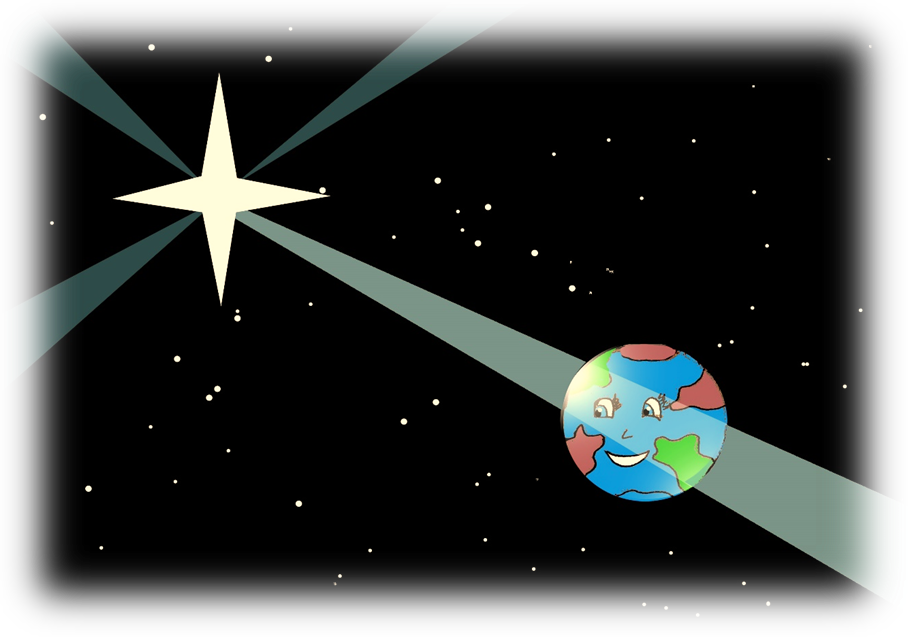
\includegraphics[width=0.85\textwidth]{estrela}
\end{figure}